\chapter{Energy Impact of Memory-Aware \\ System Scenario Approach}
\label{norchip}

\begin{center}
Iason Filippopoulos, Francky Catthoor, Per Gunnar Kjeldsberg, \\ Elena Hammari and Jos Huisken
\\
IEEE NORCHIP conference
\\
pages 1 –6, nov. 2012
\end{center}
\afterpage{\null\newpage}
\newpage

\vspace*{\fill}
\phantomsection
\section*{\hspace*{\fill} Abstract \hspace*{\fill}}
\addcontentsline{toc}{section}{Abstract}
System scenario methodologies propose the use of different scenarios, e.g., different platform configurations, in order to exploit variations in computational and memory needs during the lifetime of an application. In this paper several extensions are proposed for a system scenario based methodology with a focus on improving memory organisation. The conventional methodology targets mostly execution time while this work aims at including memory costs into the exploration. The effectiveness of the proposed extensions is demonstrated and tested using two real applications, which are dynamic and suitable for execution on modern embedded systems. Reductions in memory energy consumption of 40 to 70\% is shown.
\vspace*{\fill}
\afterpage{\null\newpage}
\newpage

\section{Introduction}
\label{sec:introduction}

Modern embedded systems are becoming more and more powerful as the semiconductor processing technique keep increasing the number of transistors on a single chip. Consequentially, demanding applications, such as medical signal processing and streaming applications, can be executed on these devices \cite{narasinga}. On the other hand, the desired performance has to be delivered with the minimum power consumption due to limited amount of power offered in mobile devices \cite{tcm}. System scenario methodologies propose the use of different platform configurations in order to exploit variations in computational and memory needs often seen during the lifetime of such applications \cite{tcm}. A platform can, e.g., be configured through frequency/voltage scaling or turning certain processing units on or off. In this work a reconfigurable memory platform is employed in order to study the effectiveness of a memory-aware system scenario methodology.

As shown in \cite{Gonzalez1996} memory contributes around 40\% to the overall power consumption in general purpose systems. Especially for embedded systems, the memory subsystem accounts for up to 50\% of the overall energy consumption \cite{Che09} and the cycle-accurate simulator presented in \cite{Ben99} estimates that the energy expenditures in the memory subsystem range from 35\% up to 65\% for different architectures. According to \cite{tcm}, conventional allocation and mapping of data done by regular compilers is suboptimal. Performance loss is caused by stalls for fetching data and data conflicts for different tasks, due to the limited size of memory and the competition between tasks. In addition, modern applications exhibit more and more dynamism. This gives a strong motivation for study and optimization of memory organisation in embedded devices with strongly dynamic application behaviour.

This paper is organized as follows. Section~\ref{sec:related} surveys related work on system level exploration and on system scenario methodologies. Section~\ref{sec:methodology} presents the chosen methodology and our novel extensions to make it applicable in a memory organisation study. In Section~\ref{sec:platform} the target platform is described while the demonstrator applications are presented in Section~\ref{sec:applications}. Results of applying the described methodology to the targeted applications are shown in Section~\ref{sec:results}, while conclusions are drawn in Section~\ref{sec:conclusion}. The main contribution of the current work is the proposal of extensions to the existing system scenario methodology, in order to take into account memory costs while performing the design exploration.  

\section{Related Work and Contribution Discussion}
\label{sec:related}

Many papers have focused on memory related optimisations, also in the presence of a partitioned and distributed memory organisation with memory blocks of different sizes (e.g. \cite{Ben00b}, \cite{Ben00c}, \cite{Mac02}, \cite{Pgk01}). However, they do not incorporate sufficient support for very dynamically behaving application codes. System scenarios allow to alleviate this bottleneck and to handle such dynamic behaviour. An overview of work on system scenario methodologies and their application are presented in \cite{Gheorghita2007}. So far memory organisation is rarely considered and not fully analysed. Furthermore, the majority of the published work focus on control variables for scenario prediction and selection. They can take a relatively small set of different values that can be fully explored. However, the use of data variables \cite{Elena2010} is required for these tasks by many dynamic systems with value ranges that make full exploration impossible. 

Authors in \cite{Pal06} present a technique to optimise memory accesses for input data dependent applications by duplicating and optimising the code for different execution paths of a control flow graph (CFG) \nomenclature{CFG}{control flow graph}. One path or a group of paths in a CFG form a scenario and its memory accesses are optimized using global loop transformations (GLT) \nomenclature{GLT}{global loop transformations}. Apart from if-statement evaluations that define different execution paths, they extend their technique to include while loops with variable trip count in \cite{Pal06b}. A heuristic to perform efficient grouping of execution paths for scenario creation is analysed in \cite{Pal07}. However, our work extends the existing solutions towards exploiting the presence of a distributed memory organisation with reconfiguration possibilities.

Reconfigurable hardware for embedded systems, including the memory architecture, is a topic of active research. An extensive overview of current approaches is found in \cite{Garcia}. The approach presented in this paper differentiates by focusing on the data-to-memory partitioning aspects in the presence of a platform with dynamically configurable memory blocks. 

\section{Extended System Scenario Methodology}
\label{sec:methodology}

The system scenario methodology is based on the observation that the workload of most systems varies significantly during their lifetime due to dynamic variation of computational and memory needs in the application code. Most of the existing design methods define the worst case execution time (WCET) \nomenclature{WCET}{worst case execution time} of the most demanding task and tune the system in order to meet its needs \cite{tcm}. Obviously, this approach leads to wasted time and memory area for tasks with lower execution time and memory requirements, since those tasks could meet their needs using fewer resources and consequentially consuming less energy. 

In contrast, designing with scenarios is workload adaptive and offers different configurations of the platform and the freedom of switching to the most efficient scenario at run-time. In contrast to use case scenario approaches in which scenarios are generated based on a user's behaviour, the system scenario methodology focuses on behaviour of the system to generate scenarios. A system scenario is a configuration of the system that combines similar run-time situations (RTSs). An RTS consists of a running instance of a task and its corresponding cost (e.g. energy consumption) and one complete run of the application on the target platform represents a sequence of RTSs \cite{Elena2010}. The system is configured to meet the cost requirements of an RTS by choosing the appropriate scenario, which is the one that satisfies the requirements using minimal power.

In the following subsections, the different steps of the system scenario methodology is outlined, with emphasis on the new extensions that make it possible to take memory into account. 

\subsection{General description of system scenario methodology}

The scenario methodology follows a two stage exploration, namely design-time and run-time stages, as described in \cite{Gheorghita2007}. The two stage exploration is chosen because it reduces run-time overhead while preserving an important degree of freedom for run-time configuration \cite{tcm}. In more detail, the application is analysed at design-time and different execution paths and variations in processing and memory demands are identified. This procedure, which is time consuming and as a result can be performed only during the design phase, will result in a grey-box model representation of the application. The grey-box model hides all static and deterministic parts of the application, by providing only related costs for those, and keeps parts of the application code that are non-deterministic available to the system designer \cite{graybox}. This way, more focus can be given to parts of the application that have impact on the cost variations so that different execution decisions can be studied. Those different options are made available to the system designer and each decision could be either fixed at design time or forwarded for dynamic evaluation at run-time.

\subsection{Design-time Profiling}

Application profiling is performed at design-time and consists of an analysis of the target application during its lifetime and for a wide range of inputs. The analysis focuses on execution time for a reference processor in the conventional system scenario methodology, but in our case the cost will be memory size. This cost metric is chosen, because several applications allocate and deallocate memory space during their execution. Also, data reuse behavior and decisions made by the system designer about the size of sets of data to be copied to different units in the memory hierarchy (i.e., copy-candidates \cite{dtse}) strongly influences the memory size. Energy consumption and access time of a memory unit is affected by its size \cite{patterson}. Together with access pattern information, the memory size is hence an important metric.

The flow of the profiling stage is depicted in Fig.~\ref{fig:profilingA} and consists of running the application code with suitable input data often found in a database, in order to produce profiling results. This reveals parts of the application code with high memory activity and with varying memory access intensity, which possibly depends on input data. Because of this behaviour, a static study of the application code alone is insufficient since the target applications for this methodology have non-deterministic behaviour that is driven by input. Choosing an extensive and accurate database is vital and will heavily influence and steer the designer's decisions in later steps.

\begin{figure}[!t]
\centering
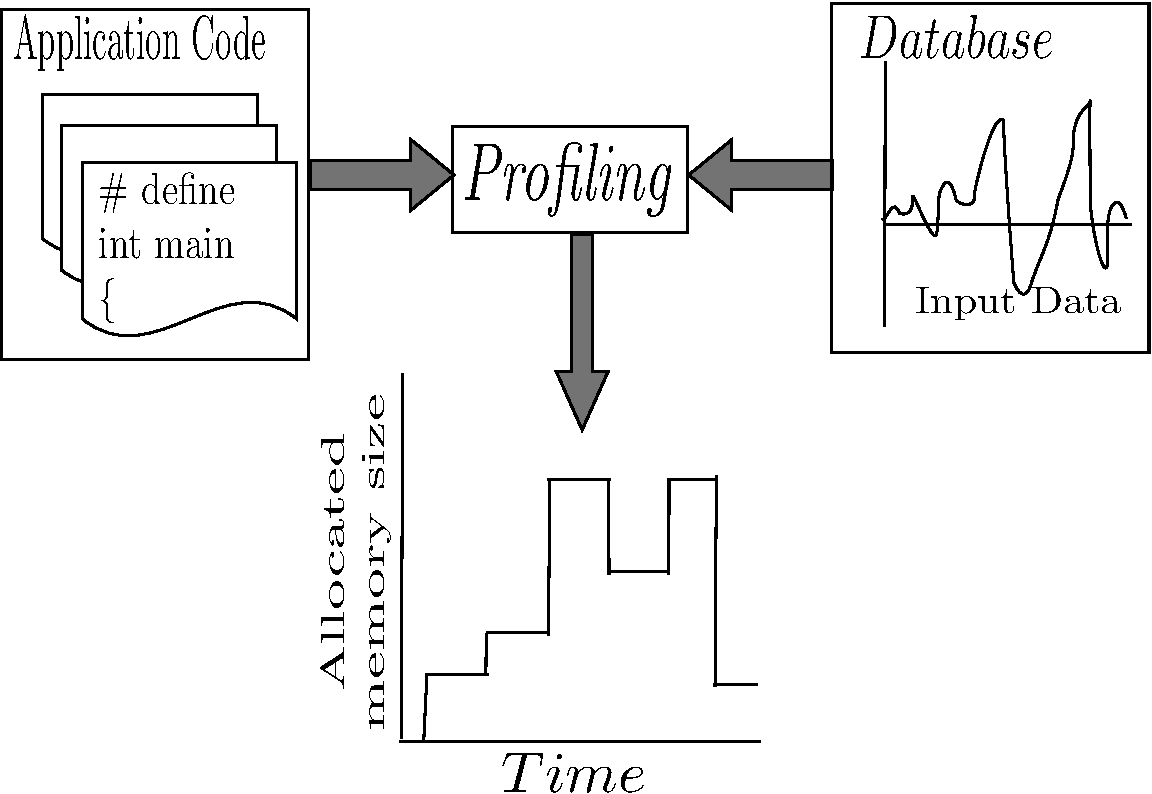
\includegraphics[width=0.8\textwidth]{A/profiling_v2-eps-converted-to.pdf}
\caption{Profiling results based on application code and input data.}
\label{fig:profilingA}
\end{figure}

Given code and database as inputs, profiling will show memory usage during execution time by running the application using the whole database as an input. Results provided to the designer include complete information about allocated memory size values together with the number of occurrences and duration for each of these memory size values. Moreover, correlation between input data values and the resulting memory behaviour can possibly be observed. This information is forwarded to the next stage.

There are several ways that profiling can be performed. Current program monitoring software cannot offer the needed level of detail. Debuggers and memory tools, such as Valgrind \cite{Valgrind}, or direct hard-coded profiling are preferable methods, because of their higher accuracy.

\subsection{Design-time Scenario Identification and Prediction}

Scenario generation is also performed during design time and is the procedure of clustering profiled information into groups with similar characteristics. More precisely, cost points are clustered in groups based on their distance in cost axis and the frequency of their occurrence. Clustering is necessary, because it will be extremely costly to have a different scenario for every possible situation. Switching cost, which is the cost of switching platform to another configuration, for example by turning a memory to retention state, grows with the number of scenarios, because more scenarios result in more frequent switching. In addition, the runtime manager becomes more complex with an increasing number of scenarios.

As shown in Fig.~\ref{fig:clusteringA}, using the information available after application profiling, situations with similar platform needs will be organised in a common scenario. This is known as clustering of RTSs \cite{Gheorghita2007}. This is a rational choice, because two instances with similar platform needs have similar memory energy consumption. The energy gain of having two dedicated scenarios is small and normally outweighed by switching costs if organized in different scenarios. In this example, clustering results in three different scenario areas (Fig.~\ref{fig:clusteringA}) and the execution scenario sequence is 1(lower), 2(middle), 3(top), 2, 3 and 1. Also, the frequency of occurrence of each instance is an important factor in scenario generation. Instances with higher frequencies normally have their dedicated scenario, to allow higher optimization, while less common instances can be clustered together in a less optimal scenario. 

In order to generate scenarios that can be implemented in realistic memory organisations, a detailed library with memory components is needed. The library should contain a variety of memory models, including different technologies and sizes, and is used to calculate scenario costs. In this work the component library is based on memory models published in \cite{Artes2011}.

\begin{figure}[!t]
\centering
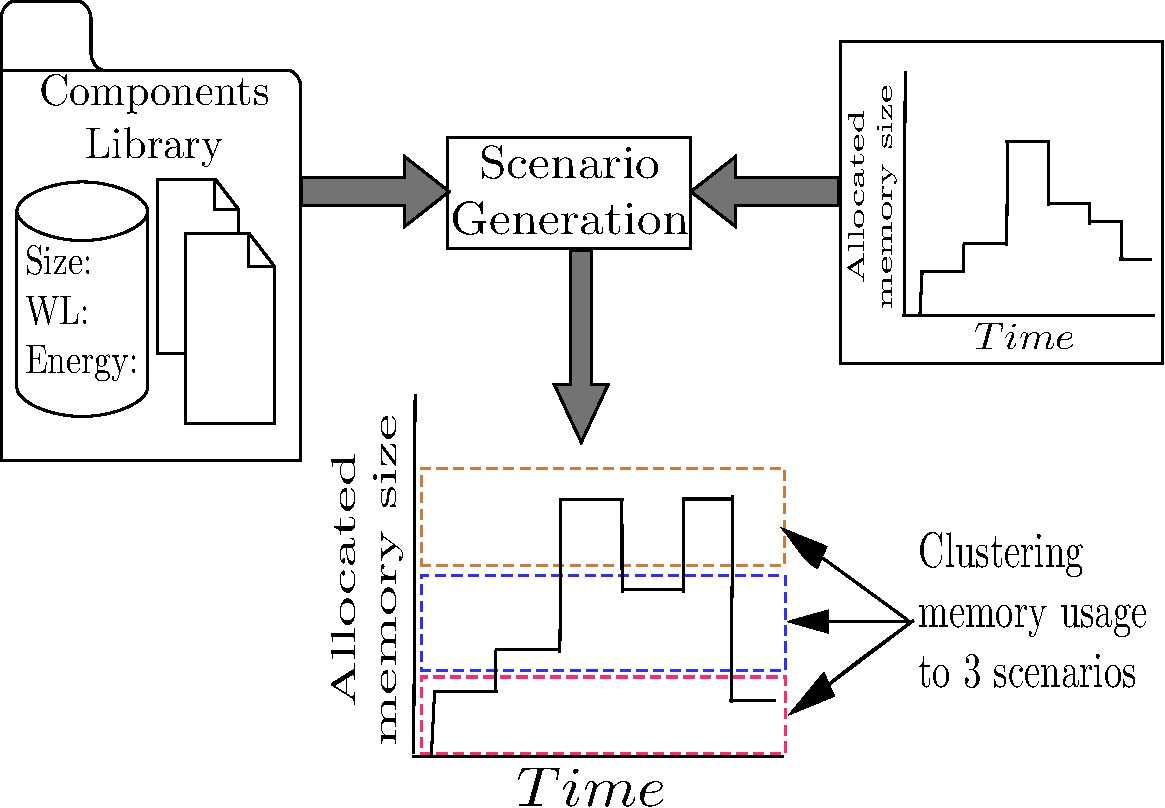
\includegraphics[width=0.8\textwidth]{A/clustering_v2-eps-converted-to.pdf}
\caption{Scenario generation based on profiling information and memory models.}
\label{fig:clusteringA}
\end{figure}

The design-time scenario prediction phase consists of determination of the variables that define the active scenario. This can be achieved by careful study of the application code, combined with the application's data input. In our case the grey-box model reveals only the code parts that will influence memory usage, so that variables deciding memory space changes can be identified. An example of this is a non static variable that influences the number of iterations for a loop that performs one memory allocation at each iteration. Moreover, the designer should look for a correlation between input values and the corresponding cost. This information will be useful in the following steps of the methodology \cite{tcm}.

\subsection{Run-time Identification, Detection, and Switching}

After profiling and scenario generation at design-time, all the necessary information needed for run-time management is available. The run-time manager monitors the current values of prediction variables selected in the previous design time step. Based on this, prediction of the next active scenario is performed  \cite{tcm}. 

Switching decisions will be taken at run-time by the run-time manager. The switching phase consists of all platform configuration decisions that can be made at run-time, e.g., frequency/voltage scaling, turning on/off a memory unit, and remapping of data on memory units. Switching takes place when the switching cost is lower than the energy gains achieved by switching. In more detail, the run-time manager compares the memory energy consumption of executing the next task in the current active scenario with the energy consumption of execution with the optimal scenario. If the difference is greater than the switching cost, then scenario switching is performed \cite{tcm}. Switching costs are defined by the platform and include all memory energy penalties for run-time reconfigurations of the platform, e.g., extra energy needed to change state of a memory unit.

\section{Target Platform}
\label{sec:platform}

Selection of target platform is an important aspect of the memory-aware system scenario methodology. The key feature needed in the platform architecture is the ability to realize different scenarios generated by the methodology. Execution of different scenarios then leads to different energy costs, as each configuration of the platform results in a specific memory energy consumption. In the conventional system scenario methodology several platform reconfiguration options have been studied \cite{Gheorghita2007} with dynamic voltage/frequency scaling (DVFS) most used \cite{dvfs}. By using DVFS techniques, one can change the frequency of the processing element and its supply voltage and energy consumption accordingly. For a memory aware scenario methodology there are multiple ways that memory reconfiguration can be performed. E.g., data can be mapped to different memory units according to size and access frequency, memory units can be turned on or off, or DVFS can be used to allow exactly the access frequency currently needed. 

\begin{figure}[!t]
\centering
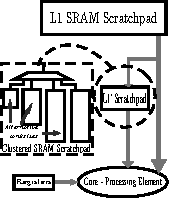
\includegraphics[width=0.8\textwidth]{A/platform_v10-eps-converted-to.pdf}
\caption{Target platform with focus on memory organisation.}
\label{fig:platformA}
\end{figure}

In this paper we have selected a relatively conventional reconfigurable architecture template that is suitable for implementing system scenarios as shown in Fig.~\ref{fig:platformA}. This dynamic memory organisation is based on memory prototypes presented in \cite{Artes2011}, and consists of two software controlled SRAM scratchpad memories, L1 and L1', and a processing element with its registers. For simplicity it is assumed that all data needed during execution is available in the L1 scratchpad memory without any time penalties even when large background memories are used. This assumption is reasonable for the kind of applications that are generally executed in embedded systems and can, e.g., be achieved through prefetching. The methodology is in general not restricted to this assumption, however, and can handle more complex hierarchical memory architectures, also including regular caches. Registers are used to save currently used elements, and between the registers and the L1 scratchpad a much smaller L1' scratchpad is introduced. This is a clustered memory that consists of four memory banks that support three different states (on, off and retention modes) \cite{Artes2011}. 

The memory energy consumption for every access in the clustered scratchpad memory is calculated based on the current situation of the platform as shown in Fig.~\ref{fig:platformA}. The leakage energy estimation is also provided in \cite{Artes2011} and is included in our study. In Tab.~\ref{tab:leakage} the leakage and wake up costs for all different operation modes are presented. The leakage in L1' is small compared to L1 and constant, thus the effect in the results is minimal.

\begin{table}[!t]
\centering
\caption{Energy costs per second and access for a reference memory bank (size: 120 bytes, technology: 90nm) in clustered L1' memory }
\label{tab:leakage}
\begin{tabular}{|c|c|c|c|c|c|c|c|}
\hline 
Modes & Leakage [J] & Wake up [J] & Access [J]\\ 
\hline 
On & $351,86 \times 10 ^{-6}$ & - & -  \\ 
\hline 
Off & $ 4,73 \times 10 ^{-6}$ & $ 2,77 \times 10 ^{-12}$ & -\\ 
\hline 
Retention & $ 97,33 \times 10 ^{-6}$ & $ 2,2 \times 10 ^{-12}$ & -\\ 
\hline 
DFF synch & - & - & $ 0.227 \times 10 ^{-6}$\\ 
\hline
DFF asynch & - & - & $ 2.18 \times 10 ^{-6}$\\ 
\hline 
Nand2 & - & - & $ 0.334 \times 10 ^{-6}$\\ 
\hline
\end{tabular}      
\end{table}

The memory energy consumption per read access is given by Equation ~\ref{eq:energyA}, which is provided by the memory models in \cite{Artes2011}.    
\begin{multline}
Read \: energy = (size \: of \: bank) \times (DFF \: sync)+ \\ + \dfrac{bank \: lines}{log2} \times DFF \: async + 4 \times size \times Nand2 
\label{eq:energyA}
\end{multline}
The cost of accessing the clustered scratchpad organisation is a function of the overall size of the cluster and the size of the specific bank being accessed. In addition, there is a contribution in energy consumption per access added by the flip-flops and the gates needed for the correct operation of the L1' memory organisation.
 
\section{Application Benchmarks}
\label{sec:applications}

The extended methodology will be tested on two representative real life applications that differentiate significantly from each other and cover different domains of applications. The first one is a computational intensive application, in which the code is dominated by loops with dynamic bounds determined by results calculated inside the loop. The second has a more static execution path, but its memory footprint is dynamically defined by the input data. Ideal applications, that can most benefit from memory-aware system scenario methodology, are applications that have dynamic behaviour in memory organisation utilization during their execution. That required dynamism could be produced by several code characteristics, covering a wide range of potential application domains for the proposed methodology.

\subsection{Epileptic Seizure Predictor}

An epileptic seizure predictor algorithm developed at Arizona State University (ASU) \cite{Iasemidis2005} is chosen as a benchmark, along with a database with measurements performed on real patients, also provided by ASU. Up to now the algorithm has only been used in clinical environments using PCs, although it would be very helpful for patients as an embedded device, as part of outpatient care. Dynamic input data dependent behaviour is identified in the algorithm and memory traces for execution of three different input samples are presented in Fig.~\ref{fig:eegprof}. For each data sample a loop is iterated 168 times. Depending on the input data sample, different memory elements are accessed in each iteration. Note that even though the element accessing for all three samples are drawn together in the figure, only one set of memory elements are accessed for each data sample and only one data sample is processed at a time. Because of the nature of the EEG \nomenclature{EEG}{electroencephalogram} signal used for the epileptic seizure prediction the benchmark has variables with a very wide range of potential values. The memory usage is heavily influenced by these input values. For demonstration purposes our study focuses on the parts of the prediction algorithm that is most dynamic. In \cite{Elena2010} the algorithm is split in thread nodes and dynamic behaviour affecting execution time is identified. The data reuse size for each sample in Fig.~\ref{fig:eegprof} contains all the elements with data reuse factor greater than 1, i.e., are read more than once. They should be saved in L1'. For example, elements in index range from roughly 3300 to 7200 for sample 1 form an approximately 3900$ \times $(element size bytes) L1' memory size requirement. These elements are read for the first time between loop iteration 0 and 50 and are also re-read later during the sample's lifetime between loop iteration 120 and 170. In Fig.~\ref{fig:eegprof} these memory elements are included in the red rectangle. The exact L1' sizes needed for processing of sample 1, 2, and 3 are 3899, 2646, and 3780, respectively.

\begin{figure}[!t]
\centering
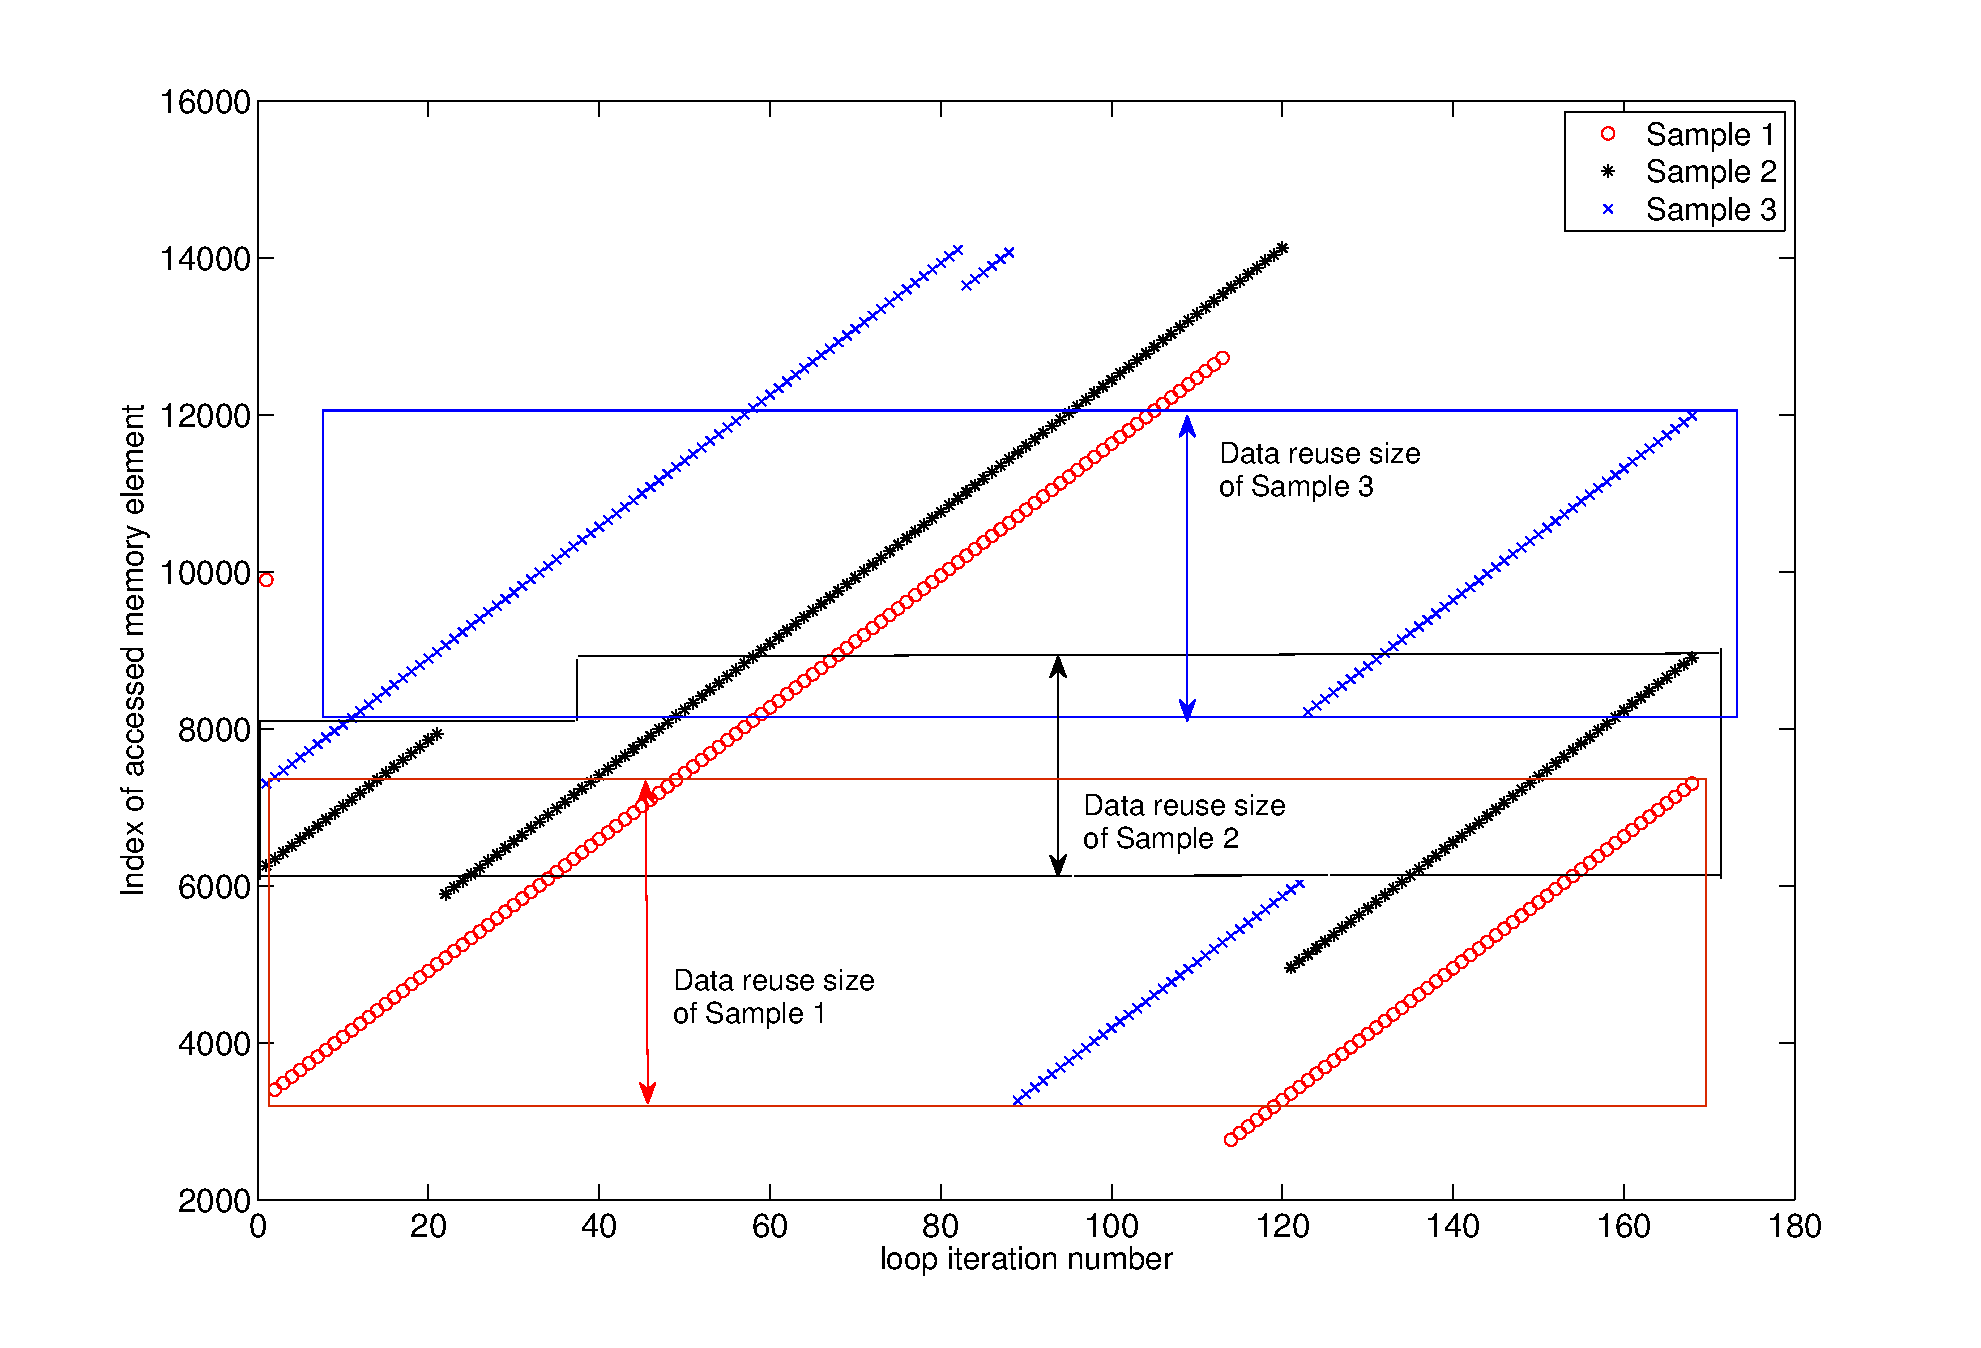
\includegraphics[width=0.8\textwidth]{A/eegprof_v1-eps-converted-to.pdf}
\caption{Memory access pattern of epilepsy predictor. Profiling of data reuse size for 3 samples from a given (\cite{Iasemidis2005}) database. The number of elements accessed is input dependent. Only those of the 16K elements accessed multiple times should be saved in L1'. The rest are accessed from L1.}
\label{fig:eegprof}
\end{figure}

Based on profiling results, scenario generation can be performed. Two possible clustering solutions are used in this paper, both of them consisting of five scenarios. In the first clustering, the range of memory indexes is split in equally sized partitions.  In the second clustering, the range is split based on occurrence frequency, so that each scenario has almost equal number of occurrences. The reconfigurable memory platform is instantiated accordingly in our target template outlined in Section \ref{sec:platform}. It contains four equal memory banks of size 975 in the first case and four banks of increasing size (195, 585, 1170, and 1950) in the second case, since smaller sizes are used more often. 

\subsection{Viterbi Algorithm Encoder}

The Viterbi algorithm \cite{viterbi} is widely used, both in the industry and academia, as an encoding/decoding algorithm for convolutional codes. As part of the encoding of the transmitted signal, redundant bits are added, which are later used by the decoder for correction of transmission errors. The output of an encoder is a function of current input bit(s) and K earlier inputs, where K is the constraint length of the algorithm. Profiling shows that the constraint length dominates the memory cost.  In Tab.~\ref{tab:snr} \cite{avd} constraint length values to achieve $ 10^{-5} $ BER are presented for different noise levels in the channel. Due to its limited range of values, the constraint length is classified as a control variable. The scenario generation is based on profiling and aims at achieving a consistent bit error rate with the minimum memory usage. If SNR \nomenclature{SNR}{signal to noise ratio} decreases, another memory bank is activated while reduction in channel noise leads to the opposite effect. The L1' sizes can be found in Tab.~\ref{tab:snr}. Clustering has been performed for K-values 5 and 6, with a resulting L1' size of 48B, and between K-values 8 and 9, with a resulting L1' size of 72B

\begin{table}[!t]
\caption{Constraint length for SNR levels on the channel (BER $ \leqslant 10^{-5} $)}
\label{tab:snr}
\centering
\begin{tabular}{|c|c|c|c|c|c|}
\hline 
SNR (dB) & K & L1' size (B) & SNR (dB) & K & L1' size (B) \\ 
\hline 
6,5 - 6,1 & 5 & 40 & 3,9 - 3,1 & 9 & 72 \\ 
\hline 
6,1 - 5,5 & 6 & 48 & 3,1 - 2,8 & 12 & 96 \\ 
\hline 
5,5 - 3,9 & 8 & 64 & 2,8 - 2,5 & 14 & 112 \\ 
\hline 
\end{tabular}      
\end{table}
 
\section{Results}
\label{sec:results}

The memory aware system scenario methodology is applied to both of our benchmark applications to study its effectiveness. Memory energy consumption is calculated based on \cite{Artes2011} and is the sum of (energy per access) $ \times $ (number of accesses) and energy costs for all transitions between memory modes. The energy for each access is defined by the type and the size of the accessed memory. Based on profiling and scenario generation results, four different memory organizations are compared for the epileptic seizure predictor. The first one is a scenario strategy without memory awareness and use a single memory bank large enough to satisfy the most demanding sample. That approach is the worst case for the memory size and statically allocates the highest value of the memory space demanded during the lifetime of the application, i.e., 3900. However, the number of accesses to the memory will be determined by each sample and no worst case assumption is made for number of accesses.

The second approach assumes that L1' has four banks of the same size (975) that can be turned on and off. The third one assumes an L1' with four banks with different sizes (195, 585, 1170, and 1950), in order to better exploit RTSs with small memory footprints.  Finally, a theoretical lower bound assumes an unlimited number of memory banks in all sizes to optimally exploit every situation. Comparison results are shown in Fig.~\ref{fig:gainsEEG} and memory energy gains up to 40\% are achieved with the scenario methodology for dynamic input samples. The high quality of our results is substantiated by the fact that our energy consumption is very close to the theoretical lower bound, even though the latter is impossible due to limited area in embedded devices.  

\begin{figure}[!t]
\centering
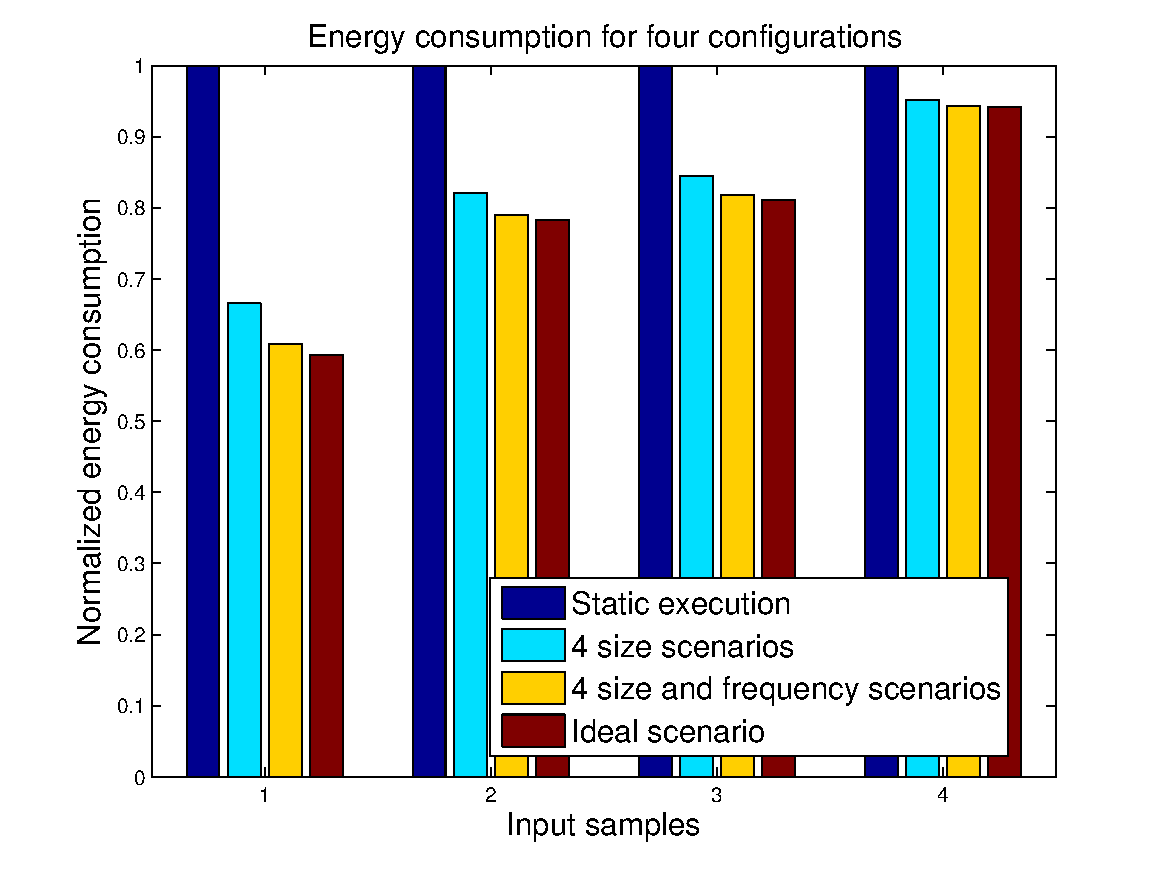
\includegraphics[width=\textwidth]{A/results1-eps-converted-to.pdf}
\caption{Memory-aware scenario gains - Epileptic seizure predictor}
\label{fig:gainsEEG}
\end{figure}

\begin{figure}[!t]
\centering
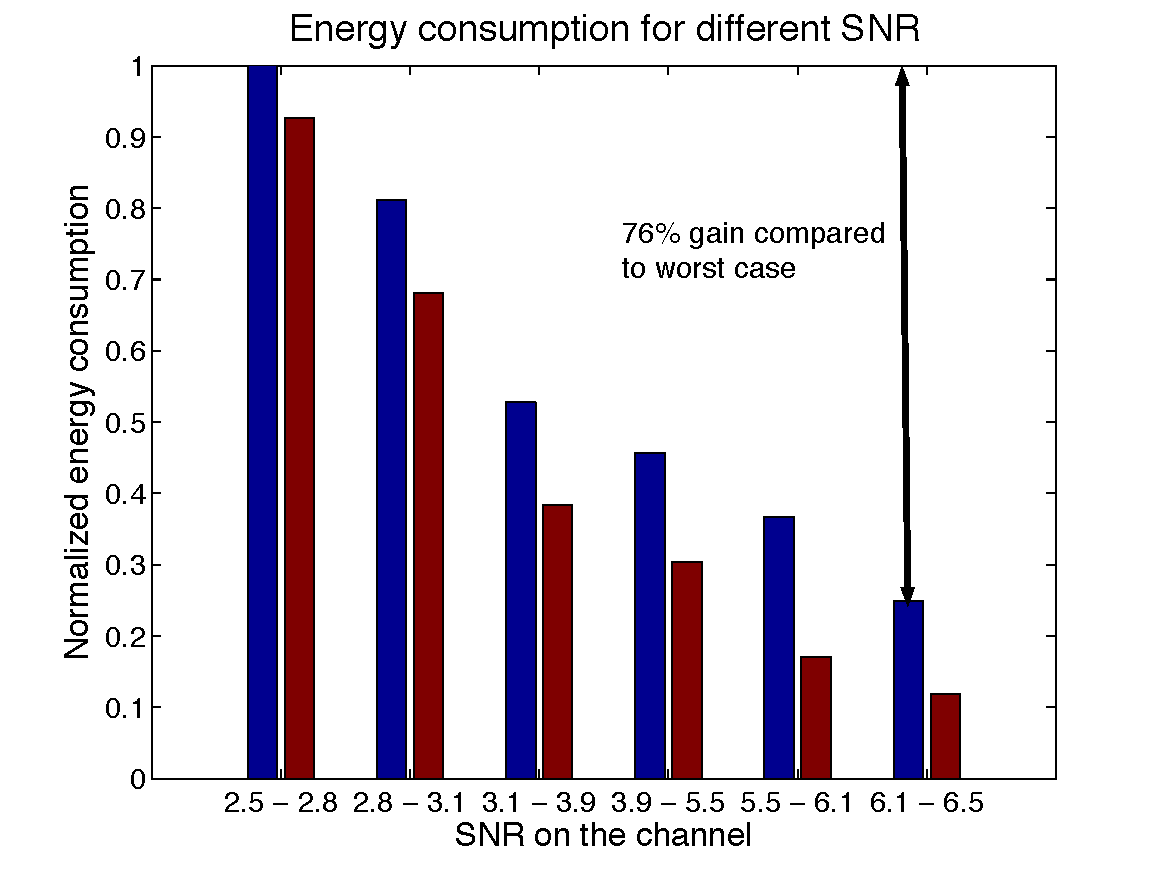
\includegraphics[width=\textwidth]{A/res2arrow.pdf}
\caption{Memory-aware scenario gains - Viterbi encoder}
\label{fig:gainsViterbi}
\end{figure}

Even higher gains are found for the Viterbi encoder (Fig.~\ref{fig:gainsViterbi}) compared to a worst-case assumption of the constraint length being equal to 14. That value of length is used to achieve acceptable BER \nomenclature{BER}{bit error rate} over very noisy channels. Using the extended system scenario methodology, L1' is split into four smaller banks that can be turned off when the noise of the channel is reduced. Again, the theoretical lower bound assumes a memory organisation with bank sizes optimized for each SNR level. Its hardware implementation would need 24 memory banks instead of 4 in our case, which leads to an unacceptable overhead. The proposed reconfigurable memory organisation can lead to more than 70\% reduction in memory energy consumption in situations with low noise, compared to a static architecture that is tuned to handle SNR levels down to 2.5 dB.

\section{Conclusion}
\label{sec:conclusion}

The scope of this work is to extend the existing system scenario techniques to better take memory into account. The memory-aware system scenario methodology has been described and tested on two real applications from bioengineering and wireless communications domains. Results justify the effectiveness of the methodology in reduction of memory energy consumption, which is of great importance in embedded devices. Since memory size requirements are still met in all situations, performance is not reduced. The memory-aware system scenario methodology is suited for applications that experience dynamic behaviour with respect to memory organisation utilization during their execution.
